% To avoid compiling stuff other than what you're working on right
% now, change the following command giving your file as its
% argument. Also, you have to modify the \input part inside the 
% \begin{document} section
%\includeonly{COCOMO}

% From now on, these are all the packages, colors and variables 
% used by all files
%%%% LAYOUT AND FONTS
\documentclass[12pt]{article}
\DeclareTextFontCommand{\emph}{\bfseries\em}

%%%% PACKAGES
\usepackage[utf8]{inputenc}
\usepackage{color}
\usepackage{caption}

% Used to specify a new tex language(Alloy)
\usepackage{listings}%

\usepackage{graphicx}
\usepackage[export]{adjustbox}
\usepackage{placeins}
\usepackage{rotating}
\usepackage{tikz}
\renewcommand{\topfraction}{.9}
\renewcommand{\bottomfraction}{.7}
\renewcommand{\textfraction}{.1}
\renewcommand{\floatpagefraction}{.66}
\renewcommand{\dbltopfraction}{.66}
\renewcommand{\dblfloatpagefraction}{.66}
\setcounter{topnumber}{9}
\setcounter{bottomnumber}{9}
\setcounter{totalnumber}{20}
\setcounter{dbltopnumber}{9}


% To split tables b/w pages
\usepackage{longtable}
\usepackage{enumitem}

%\usepackage[shortlabels]{enumerate}

%%%% GLOBAL VARIABLES
\setcounter{secnumdepth}{4}
%S: TOC Depth set to 3 as specified by Prof during lessons
\setcounter{tocdepth}{3}


%%%% COLORS
\definecolor{numbersRed}{RGB}{255, 0, 0}
\definecolor{eclipseBlue}{RGB}{42,0.0,255}
\definecolor{eclipseGreen}{RGB}{63,127,95}
\definecolor{eclipsePurple}{RGB}{127,0,85}

%%%% Actual document, remember to modify the \input part to
%%%% include your file
\begin{document}
\title{Project Plan Document}
\author{Enrico Migliorini, Alessandro Paglialonga, Simone Perriello}
\clearpage
\maketitle
\clearpage
\tableofcontents
\clearpage

\section{Introduction}
\subsection{Revision history}
\begin{longtable}{| c | c | c | c |}
	% Some table settings
	\caption{\textbf{Revision History}}
	\label{tab:rev_history}
	\\ \hline
	
	% The table itself
	\textbf{Version} & \textbf{Date} & \textbf{Authors} & \textbf{Summary}\\ \hline
	1.0 & 22/01/2017& E. Migliorini, S. Perriello, A.Paglialonga & First release\\ \hline
\end{longtable}

\subsection{Purpose and scope}
This document represents the Project Plan Document for PowerEnjoy.
The main purpose of the document is to provide a methodological estimation of the project complexity, in order to provide a guidance for the definition of the required budget, the resources allocation and the schedule of the activities.

In section \ref{sec:project-size,-cost-and-effort-estimation}, we are going to use the Function Points (\ref{sec:function-points}) and COCOMO (\ref{sec:cocomo}) approaches together to provide an estimate of the expected size of the System in terms of lines of code and of the cost/effort required to actually develop it.

In section \ref{sec:task-scheduling}, we will reuse these figures to propose a possible schedule for the project that covers all activities from the requirements identification to the implementation and testing activities.

Finally, in section \ref{sec:risk-management} we will discuss the possible risks that the System could face during the various phase of the project and provide some general conclusions.

\subsection{Definitions, Acronyms, Abbreviations}
IFPUG: International Function Point User Group

\subsection{References}
\begin{itemize}
\item RASD, DD and IT Documents for the \textit{PowerEnJoy} application
\item 
Progressive Function Point Analysis Workbook \\
available at \texttt{https://sourceforge.net/projects/functionpoints/}
\item COCOMO II Model Manual\\
available at \texttt{http://sunset.usc.edu/research/cocomoii/Docs/modelman.pdf}
\end{itemize}


\clearpage
\section{Project size, cost and effort estimation}\label{sec:project-size,-cost-and-effort-estimation}
\subsection{Size estimation function points}\label{sec:function-points}
A function point is a conceptual measure that express the amount of business functionality a software provides, based on what the end user request and receives.

The Function Points approach, originally defined in 1979 by Allan Albrecht, provides an estimation of the size of a project based.  The approach takes as inputs the functional user requirements of the software and each one is categorized into one of five types:
\begin{itemize}
	\item internal logic files (ILF) 
	\item external logic files (ELF)
	\item external inputs (EI)
	\item external outputs (EO)
	\item external inquiries (EQ)
\end{itemize} 

The 5 types of function points above, also known as Elementary Processes (EPs) can be grouped into 2 types of functions:

\begin{itemize}
	\item Inputs, Outputs and Queries all qualify as Transactional Functions and,
	\item Internal Files and External Files are distinguished as Data Functions
\end{itemize}

These groupings are helpful in determining the types of elements that each function is broken down into, to determine the complexity of the EP and ultimately the number of function points that should be awarded for a given EP.

A Transactional Function is broken down into DETs and FTRs, while a Data Function is broken down into DETs and RETs.

\begin{itemize}
	\item DET, Data Element Type is a unique user recognizable, non-repetitive field.
	\item FTR, File Type Referenced is a file type referenced by a transaction. An FTR must also be either an Internal or External file.
	\item RET Record Element Type is a user recognizable sub group of data elements within an Internal or External File.
\end{itemize}
   
Once the function is identified and categorized into a type, it is then assessed for complexity and assigned a number of function points.

\begin{longtable}{| c | c | c | c |}
	% Some table settings
	\caption{\textbf{Function Point Weights}} % Table caption
	\label{tab:fp_weights}%If later on you want to refer to this label, you can this label. 
	\\ \hline % end of row + new horizontal line
	
	% The table itself
	\textbf{Function Type} & \textbf{Low} & \textbf{Average} & \textbf{High}\\ \hline
	ILF & 7 & 10 & 15\\ \hline
	ELF & 5 & 7 & 10\\ \hline
	EI & 3 & 4 & 6\\ \hline
	EO & 4 & 5 & 7\\ \hline
	EI & 3 & 4 & 6\\ \hline	
\end{longtable}

\subsubsection{Internal Logic Files (ILF)}
PowerEnjoy has to store information related to various kind of entities in order to provide the required functionalities. All the homogeneous information are stored into different files or tables in a database. To ensure that the entities are uniquely identified inside a specific file or table we assign to each one an ID, which is unique inside the file or the table.
\bigskip

The first entities PowerEnjoy should track are surely the users; for this reason, we have a table for them storing for each one an email, a password, a social security number, a driving license number, a credit card number and a status (active/inactive). 
So, we can count 6 DETs, one for each of the data element identified above. Of course, we have to add the ID DET common to all the entities. Based on the information provided, we can thus judge that there will be only 1 RET ? meaning that all 7 DETs will be stored in a single file or Table in the database.
\bigskip

Secondly, we have to store information about areas: GPS latitude, GPS longitude, city and parking slots. The System has to manage two different kind of areas: a parking area and a charging area, the latter being an extension of the former. There are various kind of strategies to manage this kind of hierarchy at the data level; we choose to use the "single table strategy", in which the two classes of the hierarchy are mapped to a single table or file which has a discriminator column containing a value that identifies the subclass to which the instance represented by the record belongs. In our case, this discriminator is a boolean condition that is set to true if the specified record is a charging area. In addition to this field, for a charging area, we also have to add another field to store the number of charging slots associated to the charging area.\\
So, in the end we can come up with 1 RET and 7 DETs.
\bigskip

Another important piece of information is associated to the cars managed by the System. For each car, we have to store plate number, GPS latitude, GPS longitude, battery level and the status (available, unavailable, reserved or in use). We must also have a field to check if the car is plugged to a socket of a charging area. Finally, we have to know in which area the car is; for this reason, we have a field that has the identifier of an area. Thus, for this kind of data, we came up with 1 RET and 8 DETs.
\bigskip

Closely related to a car we also need a table containing all the damages. A damage, for this reason, has a mandatory identifier of the car on which the damage is. Apart from this, the table has other fields to help the identification of the damage: a text containing the description and if the specific damage is a major damage or not. It also stores two different timestamps related to when the damage was detected and when (optionally) it was solved. Of course, we have also a boolean flag that indicates if a damage has been solved or not. For this reason, we count 1 RET and 8 DETs.
\bigskip

For the main functionalities provided by our System we have to store other two different kind of homogeneous data: the first one for the reservations and the second one for the drivings.
First of all, each reservation has a reference to both the ID of the user which has made the reservation and the ID of the car being reserved. Also, we store the time on which the reservation was made and the time on which it was concluded. Finally, we have a boolean flag to know if the reservation is currently active.
We came up with 1 RET and 5 DETs.
\bigskip

The driving table is very similar to the previous one, storing a reference to both the ID of the user which driving the car, the ID of the car being driven, the time on which the drive started, the time on which it was concluded and the active flag. Apart from the previous fields, we have to store other information relevant for the evaluation of the fee applied to the user: three flag to know if the drive has to be applied a discount (the user has taken other passengers, the user left the auto with an high battery, the user plugged the car into a socket at the end of the ride) and other two for a surcharge (if the user left the auto with a low battery or if the car was left far from a charging area). In the end, we have 1 RET and 11 DETs.
\bigskip

Another homogeneous kind of data stored is related to the banking operations managed by our System. A banking operation can be related to an expired reservation or to a driving. For this reason, we have two optional data elements: the first one refers to the ID of a reservation, the last one to the ID of a driving. Of course we must also store the final fee of the specific banking operation, if it has been paid and if it has been processed. Thus, we have 1 RET and 6 DETs.
\bigskip

In the ILF we must surely count the various configuration files used by the System to define the amount of each banking operation. This kind of data relies on many different variables:
\begin{enumerate}
	\item the fee per driving minutes contains how much a user should pay for each minute of drive
	\item fee per expired reservation represents how much a user should pay for a reservation which is expired
	\item passengers discount percentage represents the percentage of the discount to be applied in the case in which the user picked up other passengers during the drive
	\item passengers number for discount is the data elements saying how many passengers a user should have picked up in order to qualify for the passengers discount
	\item passengers time for discount is the data elements saying the minimum amount of time the passengers should be in the car in order to qualify for the passengers discount
	\item high battery discount percentage represents the percentage of the discount to be applied in the case in which the user left the car with an high battery percentage at the end of the ride
	\item high battery percentage for discount  is the data elements saying the minimum battery percentage level requested to apply an high battery discount
	\item plugged car discount percentage represents the percentage of the discount to be applied in the case in which the user connected the car plug to a socket of a charging area at the end of the ride
	\item plugging car time indicates the maximum time the System waits until the user connects the plug, after which the discount is not applied anymore
	\item away from charging area surcharge percentage represents the percentage of the surcharge to be applied in the case in which the user, at the end of the ride, left the Car away from a charging area
	\item away from charging area meters represent how much is far away, id est the minimum distance between the car and the nearest charging area used to apply the surcharge at the previous point
	\item low battery surcharge percentage represents the percentage of the surcharge to be applied in the case in which the user, at the end of the ride, left the Car with a low battery percentage
	\item low battery percentage for surcharge represents the maximum percentage of the battery that has to be considered as low battery for the surcharge at the previous point.
\end{enumerate}
We don't need an ID for this kind of data, so we can easily conclude that we have 1 RET and 13 DETs.
\bigskip

The last kind of data we should manage is related to the configuration of other parameters related to the cars, namely:
\begin{enumerate}
	\item locate car nearby range, id est the maximum range between an user and the available cars that the System should use;
	\item unlock car nearby range, id est the maximum range between an user and the car he/she has reserved inside which he/she can unlock the car;
	\item battery percentage available, id est the minimum percentage level that the System should use to classify a car as available.
\end{enumerate}
We can easily came up with 1RET and 3 DETs.
\bigskip

At the end of the ILF analysis, basing on the value of the tables \ref{tab:fp_weights} and \ref{tab:ilf_complexity_matrix}, we came up with the value indicated in the table \ref{tab:ilf_weights}.

\begin{longtable}{| c | c | c | c |}
	% Some table settings
	\caption{\textbf{Complexity matrix}} % Table caption
	\label{tab:ilf_complexity_matrix}%If later on you want to refer to this label, you can this label. 
	\\ \hline % end of row + new horizontal line
	
	% The table itself
	\textbf{RETs} &	\multicolumn{3}{c|}{\textbf{DETs}} \\ \hline
	  & 1-19 & 20-50 & 51+\\ \hline 
	1 & L & L & A\\ \hline 
	2 to 5 & L & A & H\\ \hline 
	6 or more & A & H & H \\ \hline 
	
\end{longtable}

\begin{longtable}{| c | c | c |}
	% Some table settings
	\caption{\textbf{Weights}} % Table caption
	\label{tab:ilf_weights}%If later on you want to refer to this label, you can this label. 
	\\ \hline % end of row + new horizontal line
	
	% The table itself
	\textbf{Function Type} & \textbf{Complexity} & \textbf{FPs}\\ \hline
	User & Low & 7\\ \hline
	Car & Low & 7\\ \hline
	Area & Low & 7\\ \hline
	Damage & Low & 7\\ \hline
	Reservation & Low & 7\\ \hline
	Driving & Low & 7\\ \hline
	Banking & Low & 7\\ \hline
	Fees & Low & 7\\ \hline
	Cars & Low & 7\\ \hline
\end{longtable}

\subsubsection{External Logic Files (ELF)}	
Those are data used and referenced by our System but not generated and maintained by it.
	e.g. External Systems 

\subsubsection{External Input (EI)}
	elementary operations to elaborate data coming from extern environment
	e.g. calls to our app by clients: register, confirm, login/out, reserve cars, unlock cars, drive car, end ride, enable money saving

\subsubsection{External Output (EO)}
	elem ops that generates data for the ext environm. includes elaboration of data from logic files
	e.g. notify charge to user, notify company of damage, notify 

\subsubsection{External Inquiry (EQ)}
	elem ops that involves input and output. w/out significant elaboration of data from logic files
	e.g. show areas, show available cars, 

\clearpage
\subsection{Cost and effort estimation COCOMO II}\label{sec:cocomo}
\subsubsection{Brief introduction to COCOMO II}
COCOMO (COnstructive COst MOdel) is a cost estimation algorithm allowing to estimate the time, effort and money needed to develop a project. It provides an empirical non-linear model based on two series of values:
\begin{itemize}
	\item\textbf{Scale Factors}, providing a gross estimate of the effort needed for the project.
	\item\textbf{Cost Drivers}, which can be \textit{Early Design} or \textit{Post-Architecture} and are applied to the effort as a multiplier.
\end{itemize}
COCOMO was originally published in 1981, based on a study of 63 projects of varying size and languages. COCOMO II, published in 2000, extends COCOMO by savoiding several underlying assumptions, such as waterfall development and stable requirements, and separating \textit{Early Design} from \textit{Post-Architecture} effort multipliers.

The general formula for calculating the needed Person-Months is $$ PM = 2.94 \cdot Size^E \cdot \prod_{i=1}^{n} EM_i $$ where $$ E = 0.91 + 0.01 \cdot \sum_{i=1}^{5}ScaleFactor_i $$ and size is expressed in Kilo Source Lines of Code, possibly derived from Function Points.

This estimate is made after planning the architecture, so we will use the \textit{Post-Architecture} model.

\subsubsection{Scale Factors}
On the tables are marked in grey the values we believe appropriate.
\paragraph*{Precedentedness: Low}
We have never built any similar application, although the structure of the application is not different from other projects that we have worked on. Between the three of us, we have experience of Server-Client architectures, Database Management, persistency in web applications, and an extensive knowledge of algorithms.

\paragraph*{Development Flexibility: High}
Management did not impose a choice of framework, architecture or any set of constraints except the product goals. We were therefore free to choose how to build our project.

\begin{figure}[h!]
	\centering
	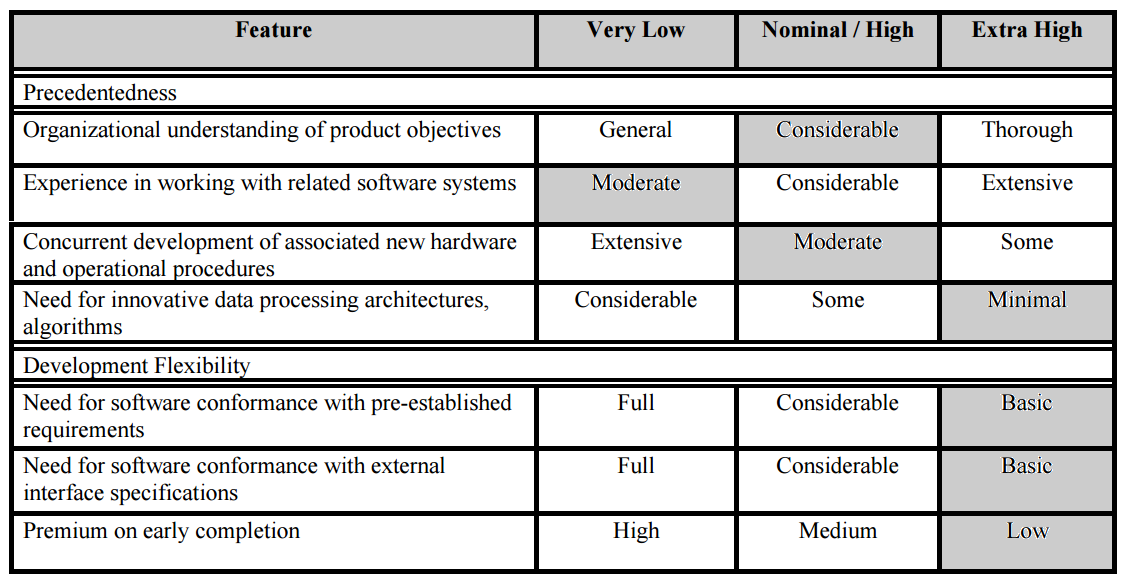
\includegraphics[width=\textwidth]{Images/PREC_FLEX}
	\caption{PREC and FLEX checklist}
\end{figure}

\paragraph*{Architecture/Risk Resolution: Low}
We were not provided with little information about risk management, budget and architecture, and had to work it out ourselves. We were allowed a high degree of freedom, and the company intervened into planning and periodic check, but we were provided little detail about the practical implementation of the preferred architectures and risk management.

\begin{figure}[h!]
	\centering
	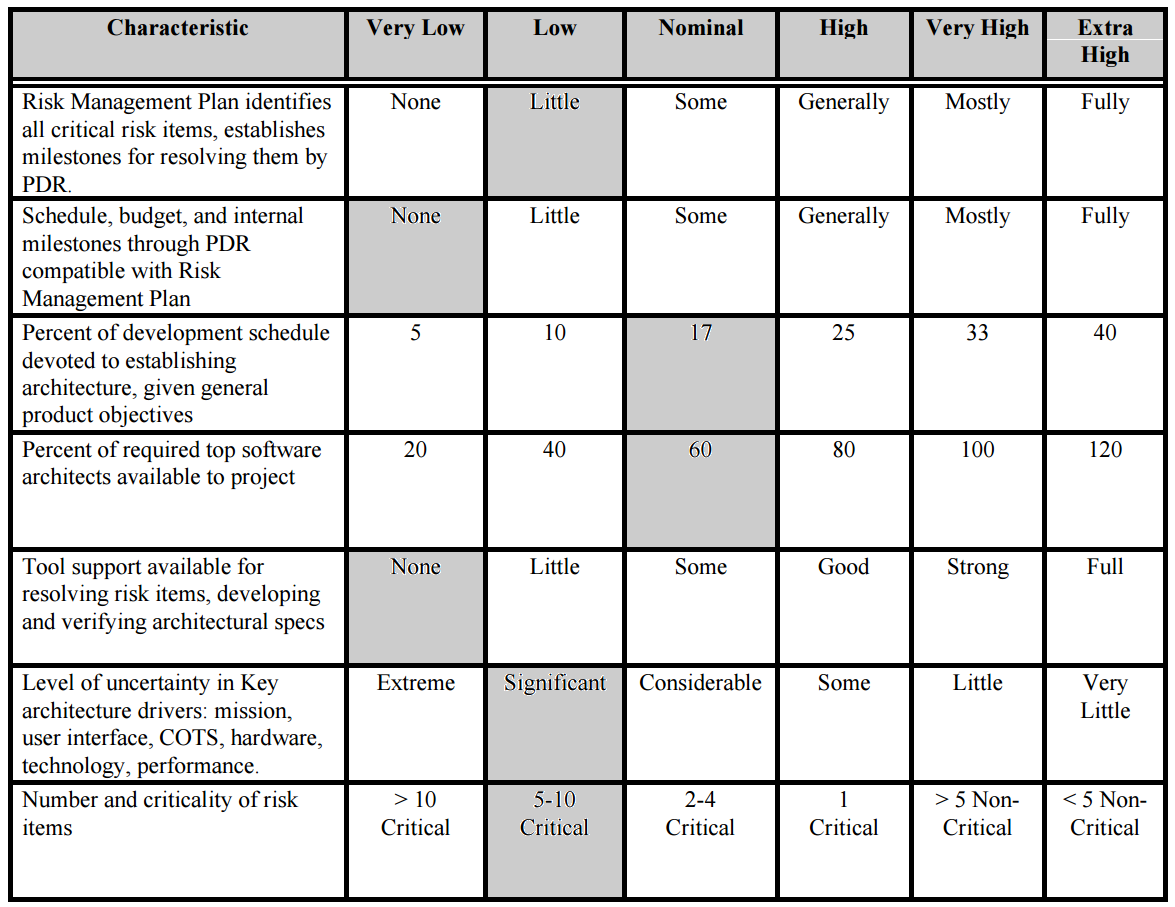
\includegraphics[width=\textwidth]{Images/RESL}
	\caption{RESL checklist}
\end{figure}

\paragraph*{Team Cohesion: High}
We had a couple of small misunderstandings early on, but managed to work them out and have been efficiently working together.

\begin{figure}[h!]
	\centering
	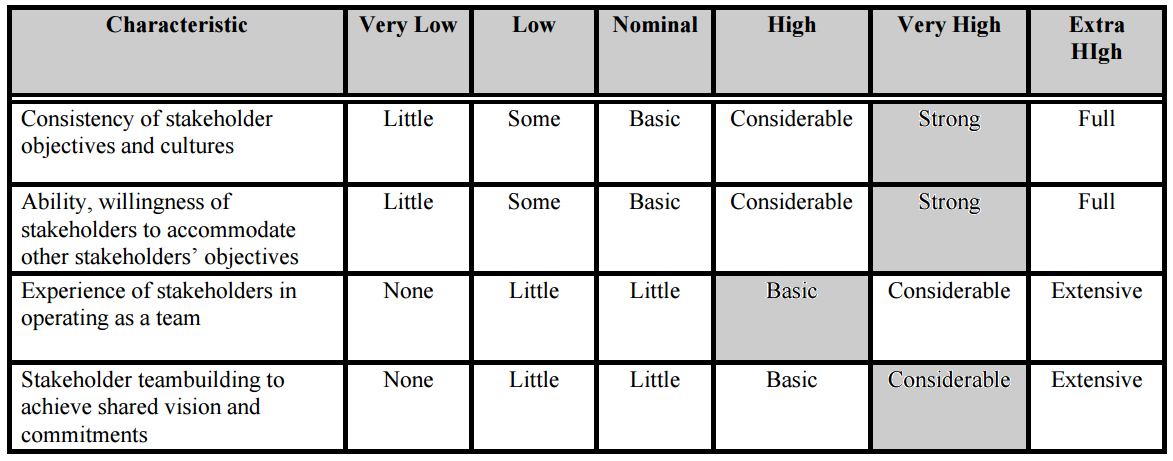
\includegraphics[width=\textwidth]{Images/TEAM}
	\caption{TEAM checklist}
\end{figure}

\paragraph*{Process Maturity: Nominal}
We believe the CMMI level to be around "Defined", accounting for our relative lack of experience but proactive attitude.

The process was managed, planned and executed by skilled people in accordance to a policy, planned together with the stakeholders, and produced controlled output. This satisfies the CMMI level 2.

In addition to that, the project was also defined at the organizational level, since our project would be the Company's main interface to the world. Additionally, we did all we could to proactively identify and address possible obstacles in the process. This satisfies CMMI level 3.

\subsubsection{Post-architecture Cost Drivers}
\paragraph*{Required Software Reliability: Nominal}
A service malfunction could cause inconvenience and non-trivial financial losses. This is because financial calculations are performed electronically, and a malfunction in the banking system could cause transaction losses. Additionally, Cars are locked and unlocked remotely, a lock service malfunction could lead to Cars being stolen.

\paragraph*{Data Base Size: Nominal}
The database size is standard for a medium-to-small-sized application. The database mainly stores data about Cars, Users, and Parking Areas. From an estimate of 12000 source lines of code, a nominal value is comprised between 120 KB and 1.2 MB, which is a reasonable estimate.

\paragraph*{Product Complexity: Nominal}
The product's complexity is par for the course for a medium-to-small-sized application. COCOMO provides a table for calculating it, which is reported and marked on the next page. The most complex part of the application is that relying on communication with the remote devices.

\begin{figure}[h!]
	\centering
	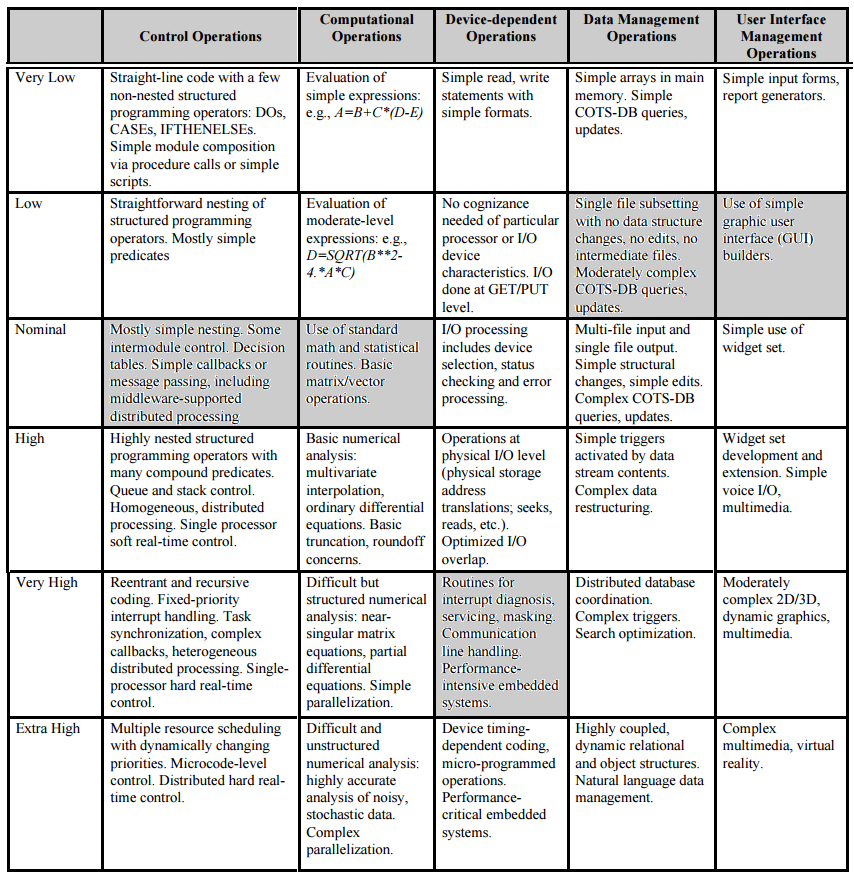
\includegraphics[width=\textwidth]{Images/CPLX}
	\caption{CPLX checklist}
\end{figure}


\paragraph*{Developed for Reusability: Nominal}
There was no specific reusability requirement, but we are working towards reusing components across the whole project whenever we do not need specialized components.

\paragraph*{Documentation Match to Lifecycle Needs: Nominal}
Adequately-sized documentation will be provided for the various stages of the project.

\paragraph*{Analyst Capability: Nominal}
We believe our skills to be around average, accounting for our relative lack of work experience. This project was designed during our course in Software Engineering 2, and we all passed Software Engineering I with good scores. We also cooperated extensively during the project.

\paragraph*{Programmer Capability: Nominal}
We believe our skills to be around average, accounting for our relative lack of work experience. We have all completed several courses of programming with good grades, showing efficiency and thoroughness,

\paragraph*{Personnel Continuity: Very High}
The three of us will keep working on the project from beginning to end.

\paragraph*{Application Experience: Low}
We have little experience in developing complete applications, but we have been working on parts of them in our previous courses. We believe 6 months' experience to be a good estimante.

\paragraph*{Platform Experience: Low}
We have little experience working with Spring, Tomcat and nginx. However, we have met several similar tools and platforms during our previous courses, so we believe 6 months' experience to be a reasonable estimate.

\paragraph*{Language and Toolset Exerience: Nominal}
We have a good understanding of Java, having used it across several courses. We are familiar with its built-in objects, main libraries, idioms, coding practices and with most Design Patterns. An estimate of 1 year's total experience is reasonable.

\paragraph*{Time Constraint: Very High}
The Central Service will consume the vast majority of the execution time, being up and running all the time (barring crashes) and tracking all the Cars In Use. So will the communication services, since rapid communication between the Cars, the User Application and the Central Service is essential for good software performance.

\paragraph*{Storage Constraint: Nominal}
No specific storage constraint was mentioned, and the amount of data created by the application is modest in size. We expect the application to use a storage percentage inferior to 50%.

\paragraph*{Platform Volatility: Low}
No major changes to any of the platforms (JavaEE, Spring, Tomcat, nginx) are expected to happen during the project, since they are all stable, mature platforms. Minor changesare expected, mostly in the form of software upgrades and patches.

\paragraph*{Use of Software Tools: High}
During development, several strong tools will be used to check on the lifecycle, such as mantaining a git repository. We will regularly update the repository with the latest source code, keeping the various design documents in the same place for easy access and accountability.

\paragraph*{Multisite Development: Extra High}
Most of the work will be done from home, coordinating through IRC and telephone. This way, there will be no time wasted in looking for a place to work together.

\paragraph*{Required Development Schedule: Nominal}
A rigid schedule was imposed on us for the first documents (RASD and DD), but we have more freedom for the project development. We will focus on concentrating our efforts in the early phases of development, in order to leave time for the unexpected.

\subsubsection{Effort Calculation}
By applying the algorithm (we used a free online tool, available at \\\texttt{http://csse.usc.edu/tools/COCOMOII.php}) based on our estimate of 236 FP, we obtained a result of 37.6 Person-Months, equivalent (considering a 160-hours work week) to 6016 Person-Hours.
\begin{figure}[h]
	\centering
	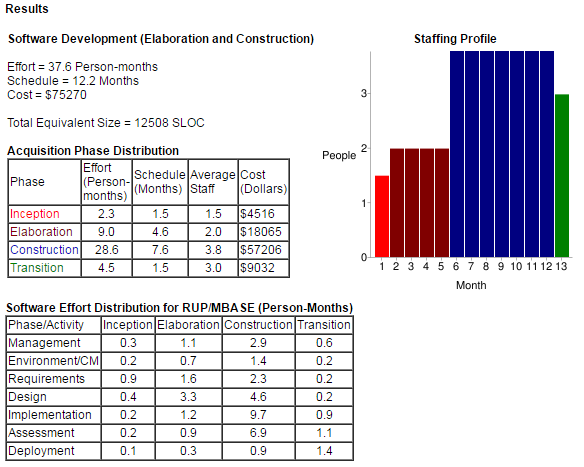
\includegraphics[width=\textwidth]{Images/COCOMO}
	\caption{COCOMO tool results}
\end{figure}

\subsubsection{Scheduling}
COCOMO provides an estimate of the project time frame through the formula $$ Duration = 3.67 \cdot Effort^{SE} $$ where $$ SE = 0.28 + 0.2 \cdot (E - 0.91) $$
resulting in an estimate of 12.2 months.

\subsubsection{Team Dimension}
The dimension of the team can be easily calculated as $\frac{Effort}{Duration}$, which, in our case, yields a result of 3.1. Since there are 3 of us, the duration will likely be extended.

This is also due to the fact that the amount of staff needed in the different phases of development is not constant: the construction phase would optimally require 4 people working. This can be avoided by hiring an additional developer, or extending the deadline. In the latter case, a realistic adjusted duration would be equivalent to 14.2 months, to reflect the increased time needed for the software construction.

\clearpage
\section{Task scheduling and resource allocation}\label{sec:task-scheduling}
For each of the required documents, we have split our tasks between ourselves. For the development of the application, we have separated a few large tasks and split them.

The following Gantt and resource diagrams show how these has been split. We are using the COCOMO-estimated development time, adjusted to reflect how our preliminary work was corresponding to the "Inception" development phase.

The redaction of the Code Inspection document was not part of the PowerEnJoy project, therefore has not been included.
\\
\\
\begin{table}[h]
\centering
\begin{tabular}{l|l|l}	
	\textbf{Major Task} & \textbf{Start Date} & \textbf{Deadline} \\ \hline
	Requirement Engineering (RASD) & 16/10/16 & 13/11/16 \\ \hline
	Software Design (DD) & 14/11/16 & 11/12/16 \\ \hline
	Integration Test (ITD) & 04/07/17 & 15/01/17 \\ \hline
	Project Planning & 09/01/17 & 22/01/17 \\ \hline
	Development & 01/02/17 & 01/04/18 \\	
\end{tabular}
\caption{Important project dates}
\end{table}

\begin{figure}[h]
	\centering
	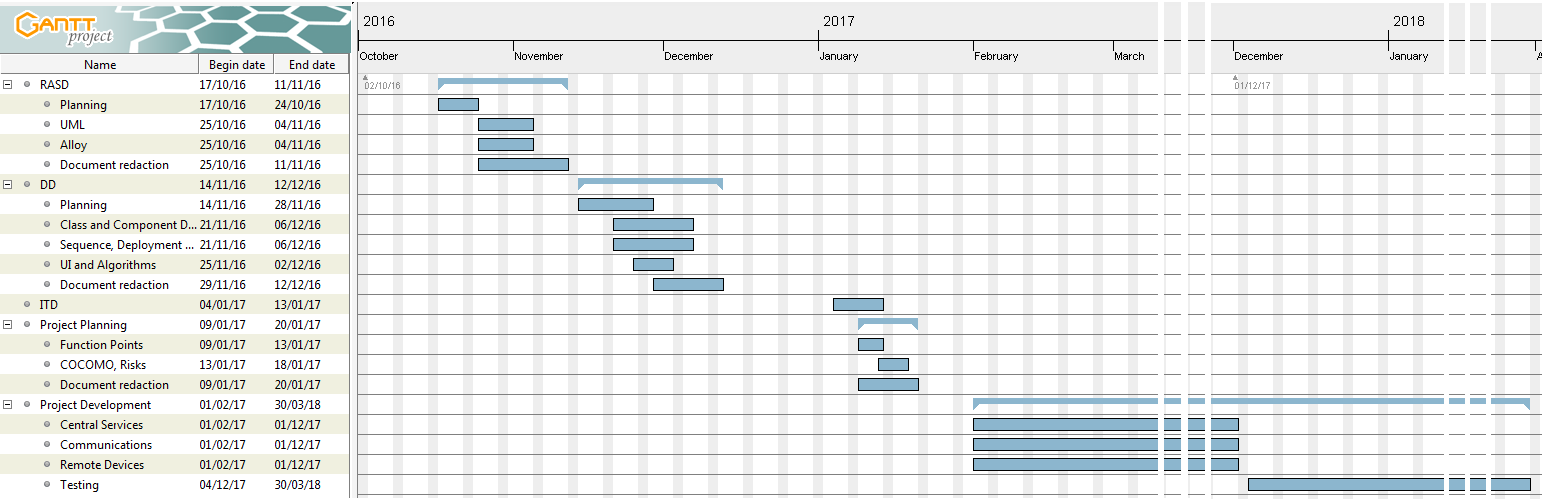
\includegraphics[width=\textwidth]{Images/GANTT}
	\caption{Gantt Diagram}
\end{figure}

\begin{figure}[h]
	\centering
	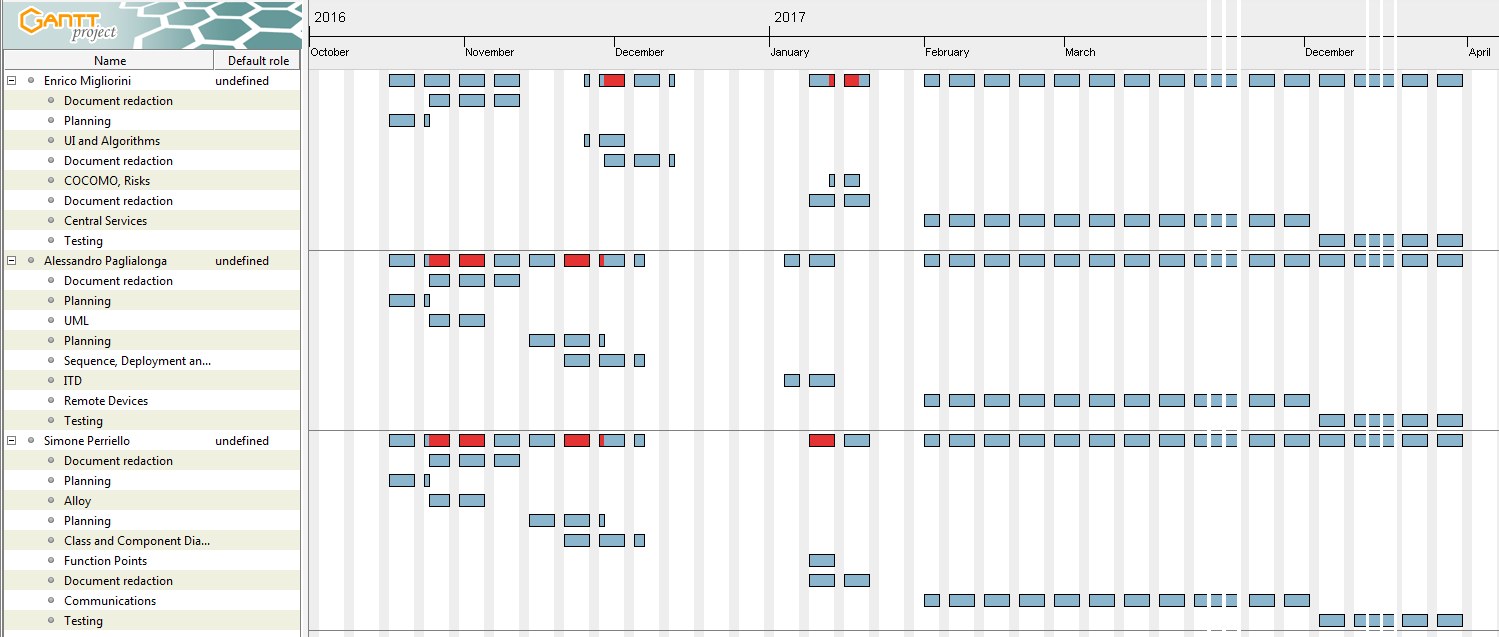
\includegraphics[width=\textwidth]{Images/RESOURCE}
	\caption{Resource Allocation Diagram}
\end{figure}

\clearpage
\section{Risk management}\label{sec:risk-management}
\subsection{Possible risks}

\begin{tabular}{|p{.07\textwidth}|p{.23\textwidth}|p{.4\textwidth}|l|l|}
\hline
\textbf{Code} & \textbf{Name} & \textbf{Description} & \textbf{Chance} & \textbf{Impact} \\ \hline
R01 & New competitors & A different company starts its own analogous service, so that our service is no longer needed. & Low & Serious \\ \hline
R02 & Client's abandonment & Client withdraws interest and funding, stopping development before release. & Medium & Critical \\ \hline
R03 & Lack of Budget & The allocated budget is insufficient to ensure development within schedule. & Medium & Serious \\ \hline
R04 & Client's modifications & Client decides to change some significant detail of the application during development. & Medium & Marginal \\ \hline
R05 & Customer's unforeseen needs & Customers need some feature that wasn't planned and included in the RASD. & High & Marginal \\ \hline
R06 & Car-Mobile communication failure & Cars and Mobile applications can't communicate properly with the Central Server. & Medium & Serious \\ \hline
R07 & Database failure & The Database is prone to errors, causing data to be unavailable or lost. & Low & Marginal \\ \hline
R08 & Server failure & The Server is prone to problems, blocking the whole system. & Medium & Serious \\ \hline
R09 & Developer's inability to work & Because of illness, personal problems or such, some of the developers can't work on the project any longer. & Medium & Critical \\ \hline
\end{tabular}

\clearpage
\subsection{Preventive strategies}
\begin{description}
	\item[R01] An accurate market analysis has to be filled out by the Client before choosing to set the project up. We can't be held responsible for the needs of the market shifting.
	\item[R02] We will require a forward payment as well as a fee for early termination.
	\item[R03] We will need to provide a realistic estimation of budget. We will need to specify in the contract that a reduction in budget will result in a sub-par product or a longer development time.
	\item[R04] We will change the product according to the Client's desires. However, we'll calculate the workload needed for these changes and warn them of the consequent increase in development time and cost.
	\item[R05] This is a problem concerning Requirement Engineering. We will set up the system so as to make it easy to expand its functionalities to accomodate any unforeseen needs.
	\item[R06] We will have to invest time and effort towards having the hardware and software needed for communication working at top performance during development. We will document extensively that area in case modifications are needed.
	\item[R07] The DBMS is external. We recommend keeping a redundant backup database in order to be able to restore functionality immediately.
	\item[R08] We will build the Server systems for parallelism, in order to minimize the consequences of a crash. Also, we'll write instructions on how to fix Server problems for the Company's IT department.
	\item[R09] We will keep some talented replacements for the missing developer(s). However, even in the best case scenario, this will extend the development time because of communications overhead.
\end{description}

\section{Work hours}
\subsection{Enrico Migliorini}
\begin{tabular}{l r}
	Day & Work hours \\
	14/01/17 & 1h \\
	16/01/17 & 4h \\
	17/01/17 & 5h \\
	18/01/17 & 3h \\
	19/01/17 & 2h \\ \hline
	TOTAL & 15h
\end{tabular}

\subsection{Simone Perriello}
\begin{tabular}{l r}
	Day & Work hours \\
	14/01/17 & 3h \\
	15/01/17 & 8h \\ \hline
	22/01/17 & 4h \\ \hline
	TOTAL & 15h \\
\end{tabular}

\subsection{Alessandro Paglialonga}
He spent 1 hour on this document, mainly due to the planning of the tasks division.
\end{document}